% INTRODUÇÃO
% - Breve introdução ao contexto e à importância da integração de dados geológicos
%   com inteligência computacional.
% - Apresente o problema que o projeto visa resolver.

\setlength{\fboxsep}{1cm}% Controla o espaçamento interno do fbox
\fbox{% Cria um box ao redor do texto
    \parbox{\textwidth}{% Permite o controle de parágrafo dentro do fbox
        \setlength{\parindent}{1.5cm} % Define a identação dos parágrafos
        \fontsize{30}{36}\selectfont % Ajusta o tamanho da fonte e o espaçamento de linha
        \textbf{Fundamentação Teórica}\\
\par{
    A coleta, armazenamento e gestão eficiente de dados geológicos formam a espinha dorsal do nosso projeto. Utilizando o PostgreSQL com a extensão PostGIS, estabelecemos uma infraestrutura robusta capaz de lidar com a complexidade e o volume crescente de dados geoespaciais. Esta infraestrutura não só permite o armazenamento detalhado de informações geológicas, mas também oferece ferramentas poderosas para sua manipulação e análise. A capacidade de realizar consultas espaciais complexas e manipular dados geográficos em tempo real é fundamental para a agilidade e precisão das análises subsequentes por modelos de IA.
}\\

\par{
    Integrando a essencial infraestrutura de dados proporcionada pelo PostgreSQL e PostGIS com a articulação sistemática de folhas cartográficas, o projeto "Da Terra ao Código" alavanca uma automação avançada no processo de predição para a exploração mineral e mapeamento geológico. Esta abordagem não só facilita o armazenamento e análise detalhada de vastos conjuntos de dados geoespaciais, mas também otimiza a geração de mapas litológicos preditivos. A implementação de folhas cartográficas no fluxo de trabalho permite a sistematização e padronização dos dados de entrada do modelo, assim como facilita as operações de requisição de dados. Esta sinergia entre a robusta gestão de dados e a integração de folhas cartográficas constitui a base para um avanço significativo na precisão e eficiência na produção de mapas litológicos preditivos para auxiliar o mapeamento geológico, assim como na produção de mapas de potencial mineral preditivos (MPM).
}\\

        \centering
        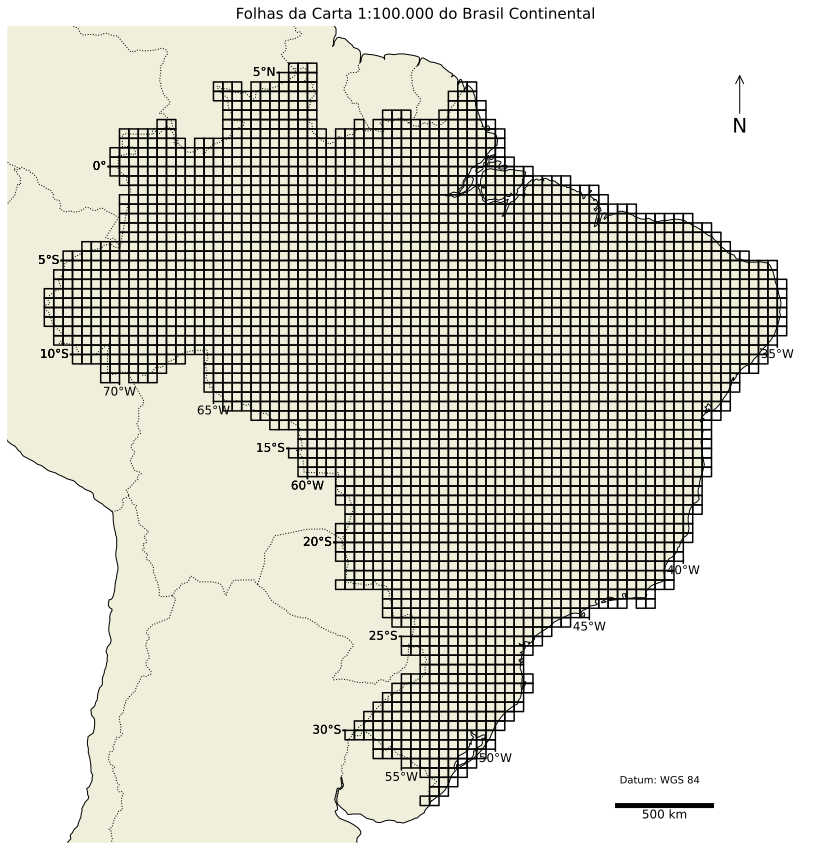
\includegraphics[width=0.9\textwidth]{../../images/100k_brasilcont.pdf}
        % Caption da imagem, legenda da figura centralizada abaixo da figura.
        \\[5mm]
        \captionof{figure}{\textbf{Representação da articulação sistemática das folhas da carta de escala 1:100.000 do Brasil continental.}}
\\[10mm]
        \justifying
        \setlength{\parindent}{1.5cm} % Define a identação dos parágrafos
\par{
    A utilização do PostgreSQL com a extensão PostGIS transforma radicalmente a gestão de dados geológicos para além das capacidades limitadas de arquivos CSV em diretórios locais. Este sistema avançado de gerenciamento de banco de dados relacional supera as abordagens convencionais ao habilitar consultas espaciais complexas e análises geoespaciais diretas, otimizando assim a integração e análise de dados para modelos de IA. Além disso, suas funcionalidades de indexação espacial e otimização de consultas garantem desempenho superior em operações de dados volumosos, enquanto mecanismos robustos de controle de acesso asseguram a integridade e a segurança dos dados. Em resumo, a escolha por PostgreSQL e PostGIS é fundamental para a eficiência, escalabilidade e precisão na exploração de dados geológicos, marcando um novo padrão em análises preditivas e no mapeamento geológico.
}
    }% fecha parbox
}% fecha fbox
